\documentclass[12pt]{beamer}
\usetheme{Warsaw}
\usepackage[utf8]{inputenc}
\usepackage[english]{babel}
\usepackage{amsmath}
\usepackage{stmaryrd}
\usepackage{amsfonts}
\usepackage{amssymb}
\usepackage{graphicx}
\usepackage{xcolor}
\usepackage[backend=bibtex, style=authoryear, maxcitenames=2]{biblatex}
\addbibresource{../../Thesis/references.bib} 
\renewcommand*{\bibfont}{\footnotesize}
\usepackage{url}
\definecolor{lila}{RGB}{128,0,128}

\newcommand{\myCite}[1]{{\scriptsize\parencite{#1}}}

\setbeamertemplate{navigation symbols}{}
\setbeamertemplate{footline}{%
	\raisebox{5pt}{%
		\makebox[\paperwidth]{%
			\hfill\makebox[10pt]{%
				\textcolor{gray}{\footnotesize\insertframenumber}
			}
		}
	}
}

\definecolor{regal}{RGB}{81,0,0}
\usepackage{array}
\usepackage{colortbl}
\makeatletter
\newcommand{\thickhline}{%
    \noalign {\ifnum 0=`}\fi \color{regal}\hrule height 4pt
    \futurelet \reserved@a \@xhline
}
\newcolumntype{"}{@{\color{regal}\hskip\tabcolsep\vrule width 8pt\hskip\tabcolsep}}
\makeatother

% listings
\usepackage[TS1,T1]{fontenc}
\usepackage{newunicodechar}
\newcommand*\longs{{\fontencoding{TS1}\selectfont s}}
\newunicodechar{ſ}{\longs}
\usepackage{listings}
\lstset{
	captionpos=b,
	frame=single,
	breaklines=true,
	tabsize=2,
	aboveskip=4pt,
	belowskip=6pt,
	literate=%
		{Ö}{{\"O}}1
		{Ä}{{\"A}}1
		{Ü}{{\"U}}1
		{ß}{{\ss}}1
		{ü}{{\"u}}1
		{ä}{{\"a}}1
		{ö}{{\"o}}1
		{~}{{\textasciitilde}}1,
	alsoletter={{\"u}}
}
\definecolor{maroon}{rgb}{0.5,0,0}
\definecolor{darkgreen}{rgb}{0,0.5,0}
\lstdefinelanguage{XML}
{
	basicstyle=\ttfamily\tiny,
	morestring=[s]{"}{"},
	morecomment=[s]{?}{?},
	morecomment=[s]{!--}{--},
	commentstyle=\color{darkgreen},
	moredelim=[s][\color{black}]{>}{<},
	moredelim=[s][\color{red}]{\ }{=},
	stringstyle=\color{blue},
	identifierstyle=\color{maroon}
}

%\setbeamercovered{transparent} 
%\logo{}  
%\subject{} 
\begin{document} 
		
\begin{frame}[plain,noframenumbering]
	\begin{minipage}{0.1\textwidth}
		\hspace{-0.5cm}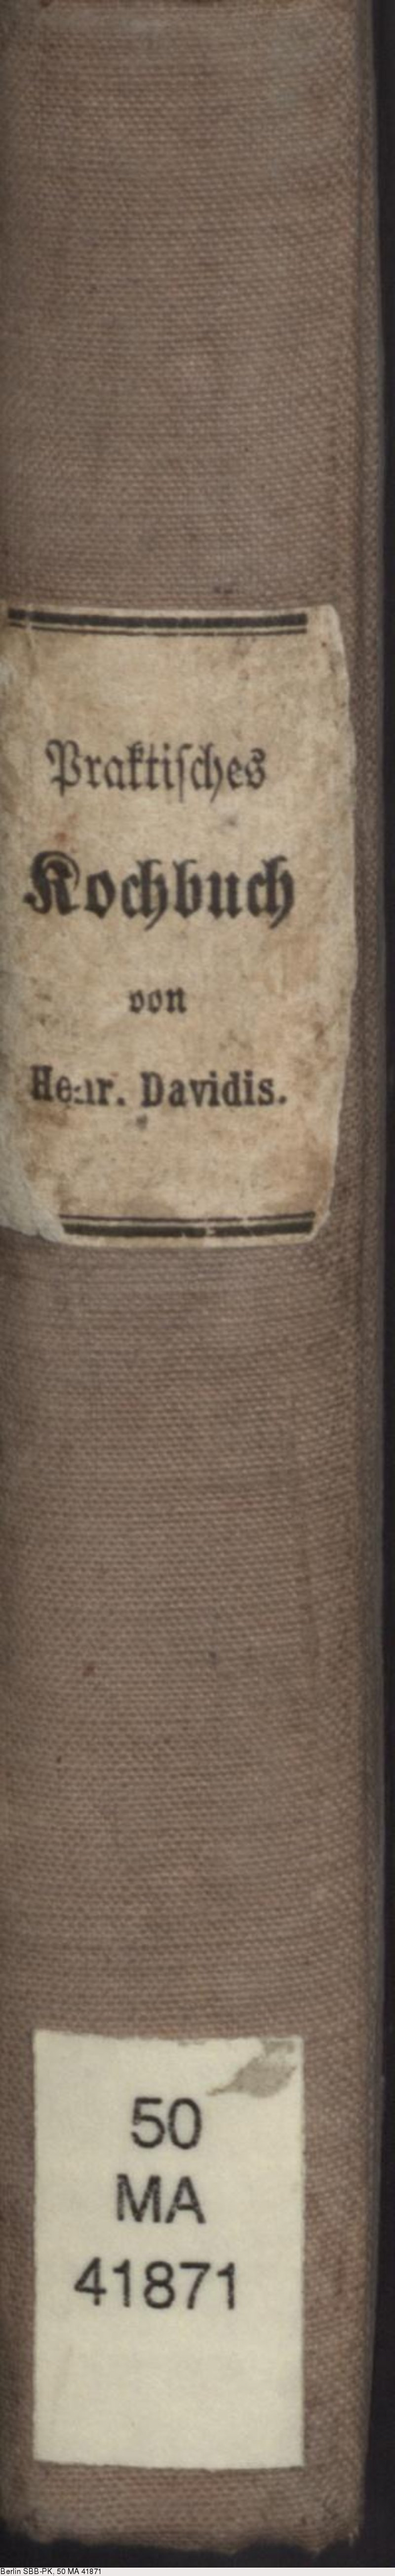
\includegraphics[scale=0.049]{Images/Buchruecken}
	\end{minipage}
	\begin{minipage}{0.6\textwidth}
		\begin{center}
			\vspace{-1.5cm}
			\Large{Extracting recipe ingredients \\ from cookbooks} \\
			\vspace{0.5cm}
			\large{Erste Schritte} \\
			\small{von \\ \vspace{-0.1cm} Torsten Knauf}
		\end{center}
	\end{minipage}
	\begin{minipage}{0.25\textwidth}
		\arrayrulecolor{red}
		\small
		\begin{tabular}{"l}
			Der Beginn einer \\ Master-Arbeit \\
			\thickhline
			\color{white} \\
			\color{white} \\
			\thickhline 
			\color{white} - \\
			\color{white} - \\
			\thickhline 
			\color{white} - \\
			\color{white} - \\
			\thickhline 
			\color{white} - \\
			\color{white} - \\
			\thickhline 
			\color{white} - \\
			\color{white} - \\
			\thickhline 
			\color{white} - \\
			\color{white} - 
		\end{tabular}
	\end{minipage}
\end{frame}

\begin{frame}
	\tableofcontents
\end{frame}

\section{Tag-Schema}
\subsection{Schema.org/Recipe}
\begin{frame}{Tag-Schema}
	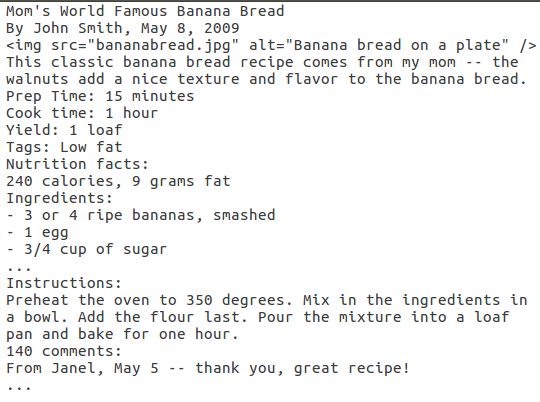
\includegraphics[width=0.7\textwidth]{Images/schemaRecipeWithoutMarkup} \\
	\myCite{schemaOrg}
\end{frame}
	
\begin{frame}{}
	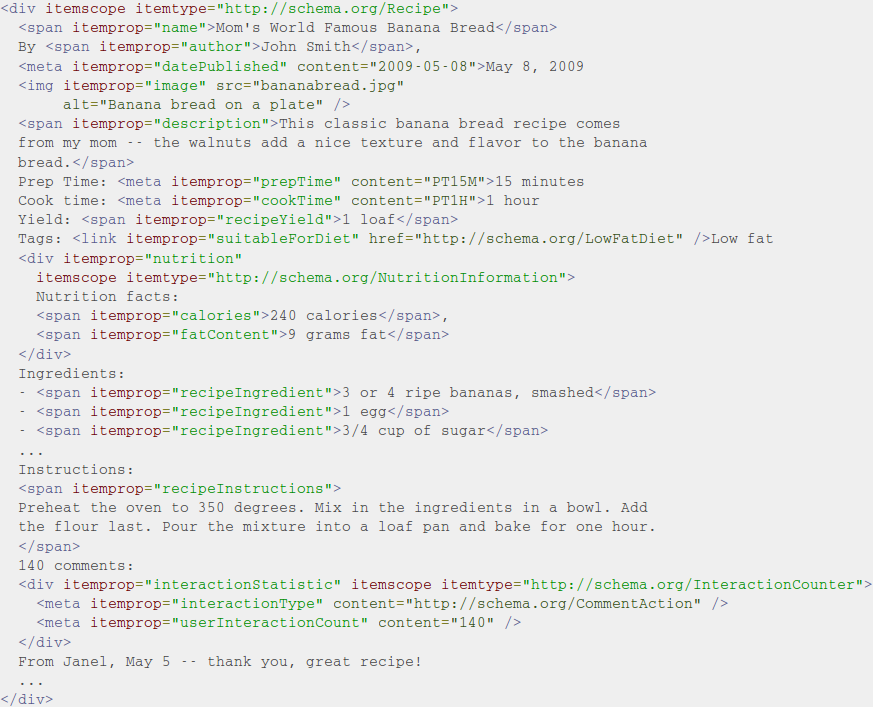
\includegraphics[width=0.95\textwidth]{Images/schemaRecipeWithMarkup} \\
	\myCite{schemaOrg}
\end{frame}

\begin{frame}{}
	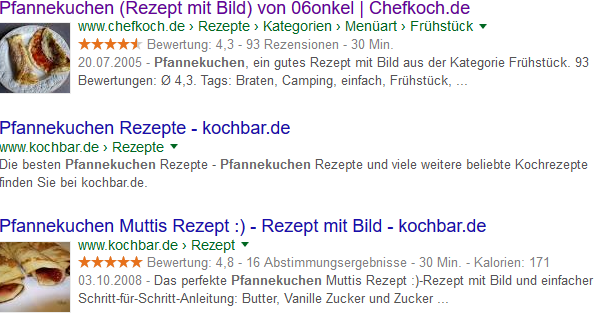
\includegraphics[width=0.95\textwidth]{Images/googleEnrichedSearchResult}
\end{frame}

\begin{frame}{}
	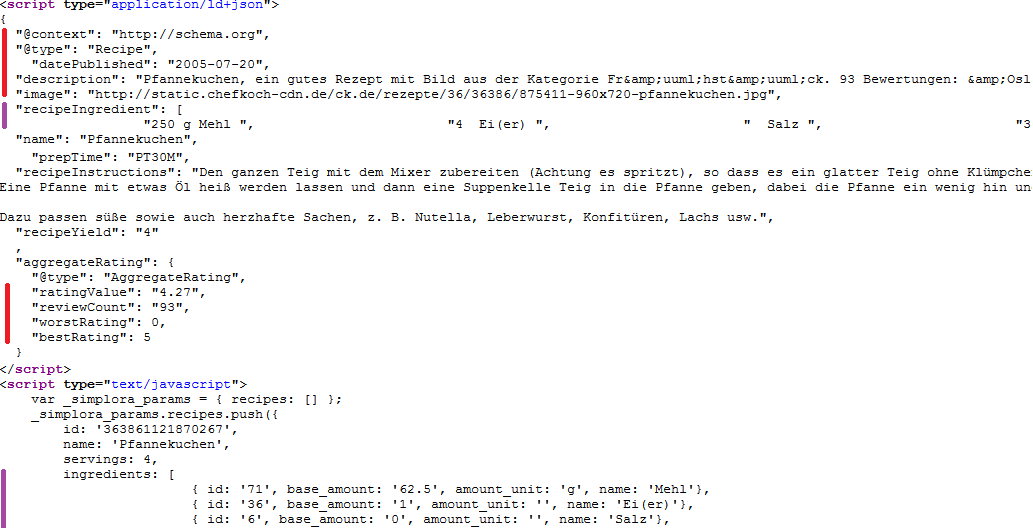
\includegraphics[width=1.4\textwidth]{Images/googleEnrichedResultJS}
\end{frame}


\subsection{cueML}
\begin{frame}{}
	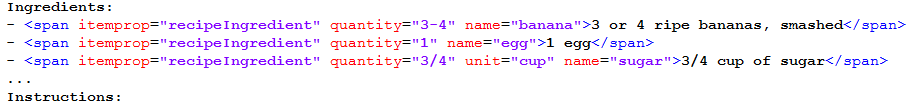
\includegraphics[width=1\textwidth]{Images/exampleCueML} \\
\end{frame}

\begin{frame}[fragile]
	\begin{lstlisting}[language=XML, caption={Beispiel Rezept von Frau Davidis}]
	<recipe type="Suppen." rcp-id="B-16">
		<head>Mock Turtle Suppe.</head>	
		
		<p>Es wird hierzu für 24-30 Personen eine kräftige Bouillon von 8-10 Pfund Rindfleisch mit Wurzelwerk gekocht. Zugleich bringt man einen großen Kalbskopf, eine Schweineschnauze und Ohren, einen Ochsengaumen und eine geräucherte Ochsenzunge zu Feuer und kocht dies Alles gahr, aber nicht zu weich. Kalt, schneidet man es in kleine, länglich viereckige Stückchen, gibt das Fleisch in die Bouillon, nebst braunem Gewürz, ein Paar Messerspitzen Cayenne-Pfeffer, einige Kalbsmidder in Stückchen geschnitten (siehe Vorbereitungsregeln), kleine Saucissen, so viel Kalbskopfbrühe, daß man hinreichend Suppe hat, und macht dies mit in Butter braun gemachtem Mehl gebunden. Nachdem dies Alles 1/4 Stunde gekocht hat, kommen noch Klöße von Kalbfleisch, einige hart gekochte Eier in Würfel geschnitten, ein Paar Eßlöffel Engl. Soja hinzu, und wenn die Klößchen einige Minuten gekocht haben, 1/2 Flasche Madeira und auch Austern, wenn man sie haben kann. Dann wird die Suppe sogleich angerichtet.</p>	
			
		<note>Anmerk. Der Soja macht die Suppe gewürzreicher, kann jedoch gut wegbleiben, und statt Madeira kann man weißen Franzwein und etwas Rum nehmen. Sowohl die Bouillon als Kalbskopf können schon am vorhergehenden Tage, ohne Nachtheil der Suppe, gekocht werden. </note>
	</cue:recipe>
	\end{lstlisting}
\end{frame}

\begin{frame}[fragile]
\begin{lstlisting}[language=XML, caption={Rezept mit cueML}]
<div itemscope itemtype="http://schema.org/Recipe http://cueML.org">
	<recipe type="Suppen." rcp-id="B-16">
		<head><span itemprop="name">Mock Turtle Suppe</span></head>
		
		<meta>
			<span itemprop="recipeYield" quantity="24-30" unit="Personen">24-30 Personen</span>
			<span itemprop="recipeIngredient" name="Bouillon" reference="#Bouillon">Bouillon</span>
			<span itemprop="recipeIngredient" name="Rindfleisch" quantity="8-10" unit="Pfund">8-10 Pfund Rindfleisch</span>
			<span itemprop="recipeIngredient">Wurzelwerk</span>
			<span itemprop="recipeIngredient" name="Cayennepfeffer" quantity="vague" unit="Messersptize">ein Paar Messerspitzen Cayenne-Pfeffer</span>
			<span itemprop="recipeIngredient" name="Ei" quantity="vague">einige hart gekochte Eier</span>
			...
			<span itemprop="recipeIngredient" name="Auster" isOptional="True">Austern, wenn man sie haben kann</span>
			<span itemprop="recipeIngredient" quantity="vague" unit="EL" isOptional="True">ein Paar Eßlöffel Engl. Soja</span>
			<recipeIngredientAlternations>
				<alt>
					<span itemprop="recipeIngredient" name="Madeira" quantity="0.5" unit="Flasche">Madeira</span>
				</alt>
				<alt>
					<span itemprop="recipeIngredient" name="weißen Franzwein">weißen Franzwein</span>
					<span itemprop="recipeIngredient" name="Rum" quantity="vague">etwas Rum</span>
				</alt>
			</recipeIngredientAlternations>
		</meta>
		<span itemprop="recipeInstructions">...</span>
	<recipe>
</div>		
\end{lstlisting}
\end{frame}

\begin{frame}[fragile]
\begin{lstlisting}[language=XML]
<div itemscope itemtype="http://cueML.schema.org/Recipe">
	<recipe type="Suppen." rcp-id="B-16">
		<meta>
			<span itemprop="name" content="Mock Turtle Suppe"/>
			
			<span itemprop="recipeYield" quantity="24-30" unit="Personen"/>
			
			<span itemprop="recipeIngredient" name="Bouillon" reference="#Bouillon"/>
			<span itemprop="recipeIngredient" name="Rindfleisch" quantity="8-10" unit="Pfund"/>
			<span itemprop="recipeIngredient" uncertainName="Wurzelwerk"/>
			<span itemprop="recipeIngredient" name="Cayennepfeffer" quantity="vague" unit="Messersptize"/>
			<span itemprop="recipeIngredient" name="Ei" quantity="vague"/>
			...
			<span itemprop="recipeIngredient" name="Auster" isOptional="True"/>
			<span itemprop="recipeIngredient" uncertainName="Engl. Soja" quantity="vague" unit="EL" isOptional="True"/>
			<recipeIngredientAlternations>
				<alt>
					<span itemprop="recipeIngredient" name="Madeira" quantity="0.5" unit="Flasche"/>
				</alt>
				<alt>
					<span itemprop="recipeIngredient" name="weißen Franzwein"/>
					<span itemprop="recipeIngredient" name="Rum" quantity="vague"/>
				</alt>
			</recipeIngredientAlternations>
		</meta>
		
		<span itemprop="recipeInstructions">...</span>
	<recipe>
</div>		
\end{lstlisting}
\end{frame}

\begin{frame}
	\begin{itemize}
		\item Das Tag-Schema ist nicht trivial, da 3 unterschiedliche Themenbereiche:
		\begin{itemize}
			\item TEI
			\item Schema.org/Recipe
			\item Information Extraction
		\end{itemize}
		\textbf{SoP (Separation of Concerns)}
	\end{itemize}
\end{frame}

\section{Algorithmen um Informationen zu extrahieren}
\subsection{RE}
\begin{frame}[fragile]{Algorithmen um Informationen zu extrahieren}
	\begin{center}
		\myCite{REgutGenug}
	\end{center}

	\begin{lstlisting}[frame=single, basicstyle=\footnotesize\ttfamily, caption={Beispiel Rezept von \newline http://recipes.wikia.com/wiki/Recipes\_Wiki}]
* Makes 6 to 8 servings

== Ingredients ==
* 2 tbsp extra virgin [[olive oil]]
* 3 cloves [[garlic]], finely chopped
[...]

== Directions ==
Heat olive oil and garlic in large skillet over low heat until
garlic begins to sizzle.
Add tomatoes, [...]

[[Category:Garlic Recipes]]
[...]
	\end{lstlisting}
\end{frame}

\subsection{CRF}
\begin{frame}[fragile]
	\begin{center}
		\textbf{Linear-chain Conditional Random Field} \\
		\myCite{CRFIntroduction}, \myCite{CRFZeit}
	\end{center}
	
	{\footnotesize Q=Quantity, U=Unit, I=Ingredient, P=Punctuation, OPT=Optional, N=Negation, O=Other}
	\begin{lstlisting}[frame=single, basicstyle=\footnotesize\ttfamily, caption={training data}]
	2 EL Zucker                     Q U I
	Einen Schuss Zucker             Q U I
	Zucker, wenn nicht süß genug    I P OPT N O O
	\end{lstlisting}
	
	\begin{itemize}
		\item \textbf{Model} $p(X,Y) = \prod_{t=1}^T p(y_t|y_{t-1}) * p(x_t|y_t)$
		\item Trainings data + Magie mit Model \\
		\quad \quad \quad \quad \quad \quad \ \textbf{$\Downarrow$}
	\end{itemize}
	
	\begin{lstlisting}[frame=single, basicstyle=\footnotesize\ttfamily, caption={Labeling}]
		2 TL Zucker                     Q U I
	\end{lstlisting}
\end{frame}

\begin{frame}
	\begin{center}
	\textbf{Model} $p(X,Y) = \prod_{t=1}^T p(y_t|y_{t-1}) * p(x_t|y_t)$
	\end{center}
	\begin{equation} \nonumber
		\begin{split}
			p(X,Y) = \frac{1}{Z(X,Y)}\prod_{t=1}^T exp(\sum_{i,j\in S}^{} \Theta_{i,j} * 1_{y_t=i} * 1_{y_{t-1}=j} + \\ \sum_{i \in S}^{} \sum_{j \in O}^{} \mu_{o,i} * 1_{y=i} * 1_{x_t=o}) 
			\\
			\scriptstyle Z(X,Y) = \sum_{X}^{}\sum_{Y}^{}\prod_{t=1}^T exp(\sum_{i,j\in S}^{} \Theta_{i,j} * 1_{y_t=i} * 1_{y_{t-1}=j} + \sum_{i \in S}^{} \sum_{j \in O}^{} \mu_{o,i} * 1_{y=i} * 1_{x_t=o}),
			\\
			\scriptstyle S = all\ possible\ labels, \quad O = all\ possible\ words
			\\
			p(X,Y) = \frac{1}{Z(X,Y)}\prod_{t=1}^T exp(\sum_{k=1}^{K} \Theta_{k} * f_k(y_t, y_{t-1}, x_t))
		\end{split}
	\end{equation}
	\small{Bemerkung: Bestimmung der $\Theta_{k}$ mathematisches Optimierungs- problem mit sehr wahrscheinlich keiner exakten Lösung}
\end{frame}

\begin{frame}
	\begin{center}
		$p(Y|X) = \frac{p(X,Y)}{\sum_{Y'\in S}^{}p(Y', X)}$ \\ \vspace{0.3cm}
		\boldmath$prediction(X) = argmax_Y(P(Y|X))$
	\end{center}
	\begin{itemize}
		\item Alles bis jetzt ist Hidden Markov Model
		\item Linear-chain CRF
		\begin{itemize}
			\item Teilmenge der $f_k$
			\item Zusätzliche custom feature functions: \\
			$f_{k+1}(y_t, y_{t-1}, X) = 1_{x_t\ starts with\ upper\ case}$ \\
			$f_{k+2}(y_t, y_{t-1}, X) = 1_{x_t\ is\ in\ a\ domain\ specific\ dictionary}$ \\
			$f_{k+3}(y_t, y_{t-1}, X) = 1_{x_t\ is\ in\ a\ domain\ specific\ dictionary *}$ \\ \hspace{3.1cm} $1_{x_{t-1}\ is\ an\ article}$
		\end{itemize}
		\item Aufwand einer Auswertung von $prediction$: $(\#S)^2*\#X$
	\end{itemize}
\end{frame}

\begin{frame}[fragile]
\begin{center}
		\textbf{Implementierung der New York Times}
\end{center}
\begin{lstlisting}[basicstyle=\small\ttfamily, frame=single, caption={Extract of the training data for New York Times CRF}]
3/4       I1  L12	 NoCAP	NoPAREN	 B-QTY
pound     I2  L12	 NoCAP	NoPAREN	 OTHER
shiitake  I3  L12	 NoCAP	NoPAREN	 B-NAME
mushrooms I4  L12	 NoCAP	NoPAREN	 I-NAME
,         I5  L12	 NoCAP	NoPAREN	 OTHER
stemmed   I6  L12	 NoCAP	NoPAREN	 B-COMMENT
and       I7  L12	 NoCAP	NoPAREN	 I-COMMENT
quartered I8  L12	 NoCAP	NoPAREN	 I-COMMENT
\end{lstlisting}
\begin{lstlisting}[basicstyle=\small\ttfamily, frame=single, caption={Feature templates}]
U01:%x[-1,0] U02:%x[0,0] U03:%x[1,0] U07:%x[0,3] U14:%x[0,1]/%x[0,2]
B
\end{lstlisting}
\end{frame}

\begin{frame}
	\begin{itemize}
		\item Über 130.000 labelled ingredient phrases
		\item 89\% sentence-level accuracy
		\item Getestet mit 481 ingredient phrases
		\begin{itemize}
			\item Nicht eindeutig: \\
			\textit{1 garlic clove, minced (optional)}
			\item Mehrere Zutaten in einer ingredient phrase nicht vorgesehen: \\
			\textit{4 tablespoons melted non-hydrogenated, melted coconut oil or canola oil}
			\item Fehler vom Algorithmus oder vom Menschen?
		\end{itemize}
	\end{itemize}
\end{frame}

\subsection{Dictionary-based}
\begin{frame}
	\begin{center}
		\textbf{Ingredient Action relationship} \\
		\myCite{GrammaBased}
	\end{center}
		
	\begin{enumerate}
		\item Dictionary-based entity recognition
		\begin{itemize}
			\item Morphologisch Analyse der Wörter (z.B. Eier $\rightarrow$ Ei)
			\item $Wort \in Domain\ specifiy\ dictionary?$
		\end{itemize}
		
		\item Welche entities gehören zusammen?
		\begin{itemize}
			\item Rule based: POS + context free grammar
			\item Dependency based
		\end{itemize}
	\end{enumerate}
	
	\begin{itemize}
	 \item \hspace{-2cm} \begin{table}[H] \vspace{-1cm}
		\centering
		\begin{tabular}{ l | c | r } 
			& Precision & Recall \\
			\hline
			Rule based & 97.39\% & 51.54\% \\
			Dependency Based & 95.4\% & 64.12\% \\
		\end{tabular}
	\end{table}
	\end{itemize}
\end{frame}



\section{Schwerpunkt setzen}
\begin{frame}{Schwerpunkt setzen}
	\begin{itemize}
		\item Schema.org/Recipe erweitern
			\begin{itemize}
				\item Via GitHub
				\item Offensichtlich Bedarf (Chefkoch, NYT)
			\end{itemize}
		\item Algorithmus
		\begin{itemize}
			\item Keine 130.000 Trainingsdaten vs. bessere feature functions (domain-specific dictionary check)
			\item Decision tree ($if\ negationWord \in X...$)
		\end{itemize}
		\item Webseite
		
		\vspace{0.5cm}
		\item Ende Februar / im März nur noch schreiben
	\end{itemize}
\end{frame}

\section{}
\begin{frame}
	\begin{minipage}{0.5\textwidth} 
		\begin{itemize}
			\item SoP (Separation of Concerns)
			\item Martin Fowler: Duplizierter Code ist die Nummer eins der Gestanksparade
			\item Agile manifest: Simplicity --the art of maximizing the amount of work not done-- is essential
			\item Praktiken von XP: Simple Design, consider the simplest thing that could possible work \& YAGNI (You aren't gonna need it)
		\end{itemize}
	\end{minipage}
	\begin{minipage}{0.48\textwidth} 
		\vspace{1cm}
		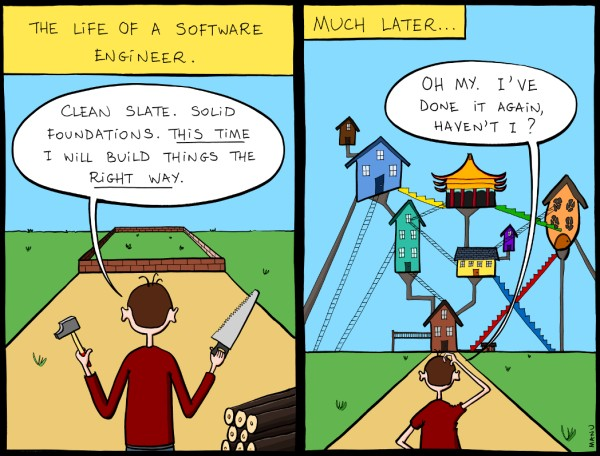
\includegraphics[width=1\textwidth]{Images/software-eng} \\
		\vspace{-0.7cm}
		\begin{center}\Large Danke für die \\ Aufmerksamkeit \end{center}
	\end{minipage}
\end{frame}


\section{}
\begin{frame}[t,allowframebreaks]{Literaturverzeichnis}
	\printbibliography[heading=none]
\end{frame}

\end{document}